\documentclass[12pt]{report}



\usepackage{graphicx}

\title{\textbf{A REPORT ON SIMCARD REGISTRATION}}
\author{MPUUGA FAIZO 14/U/9319/EVE 214004093}
\begin{document}
\maketitle


\section{Introduction} 
\paragraph{Given the Uganda Communications Commission recent issued order for all its customers to re-register their simcards using details on thier national ids, many have achieved beating the deadline for the activity but neverthless, the majority failed and thus thier simcards disconnected. }


\section{Background}
\paragraph{For the past years in Uganda, crime rate was too high characterised by unsuspected murders of important characters in the country like muslim clerics and high ranking officials. Even after notification to the police, it could do nothing big about it because it hardly had details about its nationals so it could not trace and come to a conclusion for the different crime occassions thus issuing an order for all UCC customers to re-register their simcards with their national id details.}


\section{Problem statement}
\paragraph{Despite the UCC order, the time that was situated for Ugandans to accomplish that activity was really too minimal to the extent that even after an additional time of a month, many have not yet re-registered their simcards.}

\section{Objectives}
\paragraph{The main objective for carrying out this data collection activity was to tell and provide how much time is really appropreate and sufficient for the whole process to cover up all UCC customers in uganda.}

\section{Data collection methods}
\paragraph{An open data kit was used during the process and some of the data that was collected includes; audios, photos, closed-ended questionnaires among the many.}

\subsection{Below includes some of the screenshots for the application.}
\title{images}
\maketitle
Here is a piechart of people who have and those that have not yet registered thier simcards
\includegraphics{capture.png}

A bar graph for thier reasons
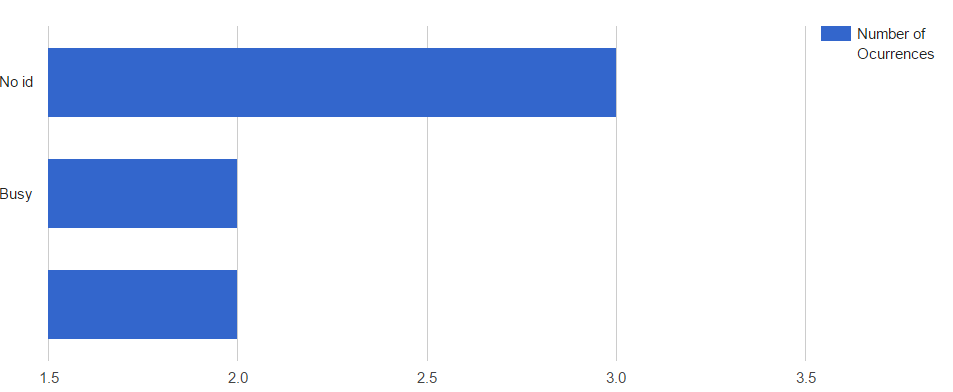
\includegraphics{graph}

\section{Conclusion}
\paragraph{Basing the collected data and after analysing it critically, most of the customers that were disconnected and those that have not yet registered are using MTN. The main reason given by those who have not yet registered is that they have not yet got thier national ids, thus signalling a direct action for the government and the UCC to prolong the re-registration activity for a full year hence giving appropreate time to those that have not yet proccessed their national ids to do so thereafter register their lines. }


\end{document}
